\section{Methods}

% model architecture

The architecture of the model is meant to resemble the hippocampal formation.
It is composed of an input area, being layer III of the entorhinal cortex (EC) with activation $\textbf{x}_{\text{ECin}}$; two hidden layers $\textbf{x}_{\text{CA3}},\;\textbf{x}_{\text{CA1}}$, representing CA3 and CA1; and an output $\textbf{x}_{\text{ECout}}$ being layer IV of EC.
In particular, it is identified an inner loop $\text{ECin}\to \text{CA1}\to \text{ECout}$ that forms an autoencoder structure, and an outer loop $\text{ECin}\to \text{CA3}\to \text{CA1}\to \text{ECout}$, as showed in figure \ref{fig:fig1}-\textbf{a}.

The neurons of each layer are artificial nodes, and the forward propagation follows the usual linear combination of the input, connections weights and a bias vector.
Concerning the activation function, we defined a modified sigmoid with a sparsity feature, relying on a parameter $\beta$; see \ref{app:sparsemoid} for details.

The training protocol is defined in two stages.
Firstly, the inner loop is trained to match the input pattern $\textbf{x}_{\text{ECin}}$ with the output $\textbf{x}_{\text{ECout}}$ using backpropagation and the Adam optimizer, as a proper autoencoder.
The goal of this passage is to imprint the connections $\textbf{W}_{\text{ECin}\to \\text{CA1}}$ with the information for compressing the entorhinal pattern, and the output connection $\textbf{W}_{\text{CA1}\to \\text{ECout}}$ with decoding abilities.

Then, in the second stage the outer loop is involved, recruiting the CA3 projections to CA1.
The trained autoencoder connections are frozen, and the focus is placed on the $\textbf{W}_{\text{CA3}\to \text{CA1}}$ connections.
Here, training occurs in the form of synaptic plasticity, and relies on the $\text{ECin}$ input, identified as the instructive signal (IS), and the CA3 activity, designated to be the eligibility trace (ET).
The goal of this stage is actually mimick the process of memory consolidation and retrieval, taking care of preserving the deconding of the the neural traces despite continuosly memorizing new patterns.
Moere specifically, the learning process is aimed at strengthen the CA3-CA1 synapses that would allow the outer loop, without the $\text{ECin}-\text{CA1}$ projections, to reproduce the input activation.
The role of the IS is thus to provide of mask over the CA1 neurons, highlighting those whose activity would more reliably preserve the input when propagate to $\text{ECout}$.

Importantly, the set of patterns used in the two stages are samples from the same distribution, such that the inductive biases developed during from the autoencoder training can guide the selection process enacted by IS.

The specific formulation of the learning rule is inspired by BTSP, in that it solely depends on IS ($\textbf{x}_{\text{ECin}}$) and ET ($\textbf{x}_{\text{CA3}}$) while discarding the post-synaptic activation $\textbf{x}_{\text{CA1}}$:

\begin{equation}
    \textbf{W}_{\text{CA3}\to\text{CA1}} = (1-\textbf{x}_{\text{ECin}}*\alpha) * \textbf{W}_{\text{CA3}\to \text{CA1}} + \alpha * (\textbf{x}_{\text{ECin}} \cdot \textbf{x}_{\text{CA3}})
\end{equation}

\noindent The hyperparameter $\beta$ effectively functions as a learning rate, modulating the integration of the new signal into the previous state of the connections.

Similarly to other accounts of the BTSP rule, the strenghtening and weakening of synaptic weights is influenced by the relative timing of the input activations it relies on.
In particular, synaptic potentiation takes place in the case of temporal coincidence, but also factoring in the magnitude of the current weight value. In fact, above a certain threshold synaptic depression takes on regardless of the relative timing.
In our context, given the discrete nature of the plasticity training protocol during the second stage, the partition of the kernel landscape is also markedly discrete, as visualized in figure \ref{fig:fig1}-\textbf{b}.


% description of BTSP

\begin{figure}[h]
    \centering
    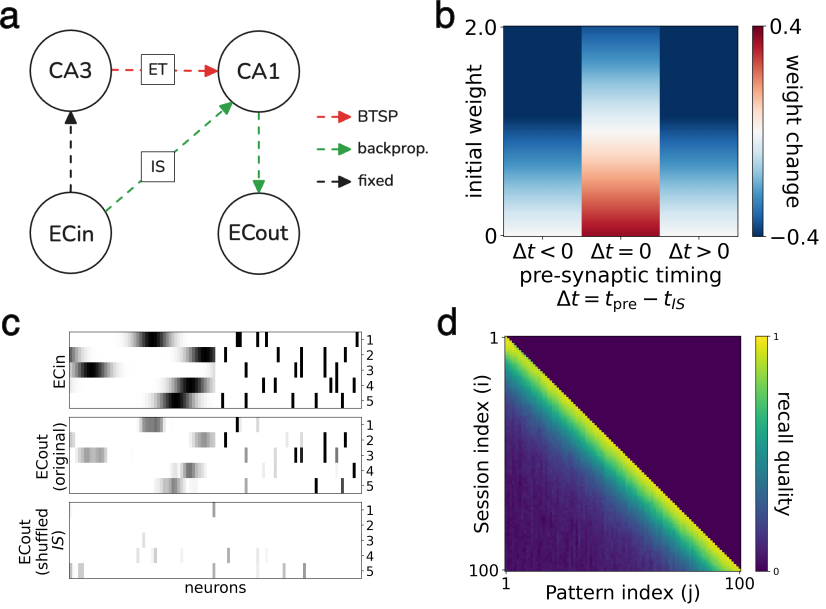
\includegraphics[width=0.9\textwidth]{figures/main_fig_a.png}
    \caption{\textsc{Figure 1} - \textbf{a}: \textit{architecture, composed of two input/output entorhinal layers and two hidden hippocampal layers}.
        \textbf{b}: \textit{kernel of the weight update resulting from the plasticity rule, blue represents synaptic depression while red synaptic
    potentiation}.
\textbf{c}: \textit{reconstruction of the} $\text{EC}_{in}$\textit{ input pattern from a model with IS intact (original) and shuffled}.
\textbf{d}: \textit{recall quality for all memories }$j$\textit{learned before pattern }$i$.}
    \label{fig:fig1}
\end{figure}




